\section{Security Assessment}
\label{appendix:security}
\subsection{A. Risk Identification}

\subsubsection{Asset Identification}

We have the following assets in our system:

\begin{itemize}
    \item Web application
    \item GitHub repository
    \begin{itemize}
        \item Public repository available for all to see
    \end{itemize}
    \item Digital Ocean servers
    \begin{itemize}
        \item Includes our database
        \item All have public IP addresses
    \end{itemize}

    \item Tools:
    \begin{itemize}
        \item Grafana
        \item Docker
        \item Docker compose
        \item Docker Swarm
        \item Pulumi
        \item Ansible
        \item Sonar Cloud
        \item Code climate
        \item Linters
        \item Loki
        \item Github Actions
    \end{itemize}
\end{itemize}

\subsubsection{Threat Source Identification}

We have taken the OWASP top 10 to help identify possible threats in the system:

\begin{itemize}
    \item Broken Access Control (OWASP no. 1)
    \item Injection attacks (SQL, etc.) (OWASP no. 3)
    \item Cryptographic failures (e.g. in password hash) (OWASP no. 2)
    \item Security misconfiguration (OWASP no. 5)
    \item Insecure Design (OWASP no. 4)
    \item Vulnerable and outdated components (OWASP no. 6)
    \item Identification and authentication failures (OWASP no. 7)
    \item Software and Data integrity failures (OWASP no. 8)
    \item Security Logging and Monitoring Failures (OWASP no. 9)
    \item Server Side Request Forgery (OWASP no. 10)
\end{itemize}

\subsubsection{Risk Scenario Construction}

Based on the information gathered from step 1 and 2, we have constructed the following risk scenarios:

\begin{enumerate}
    \item Attacker constructs URL in the \textbf{web application} with user ID such that they bypass login and can write messages from another user's account.
        \begin{itemize}
            \item Broken Access Control
            \item Server Side request forgery???
        \end{itemize}
    \item Attacker can forge log content in the **web application** to prevent an organization from being able to trace back malicious activities.
    \begin{itemize}
        \item Security Logging and Monitoring Failures
        \item Injection attack
    \end{itemize}
    \item Attacker brute forces login credentials in the **web application** by taking advantage of no timeouts + weaker hash implementation
    \begin{itemize}
        \item Cryptographic failures
        \item Identification and authentication failures
    \end{itemize}
    \item Attacker identifies weak or outdated tool in CI/CD pipeline via public **GitHub Actions**
    \begin{itemize}
        \item Vulnerable and outdated components
        \item Software and Data integrity failures
    \end{itemize}
    \item Attacker scans **public IP address** of our serves and finds unnecessarily/unexpectedly open ports with known vulnerabilities on. Exploits those vulnerabilities.
    \begin{itemize}
        \item Security Misconfiguration
    \end{itemize}
    \item SQL-Injection attacks at login-page on the **web application** targeting user database.
    \begin{itemize}
        \item Injection attack
    \end{itemize}
    \item Attacker gets access to secrets written into the public GitHub repository.
    \begin{itemize}
        \item Identification and authentication failures
        \item Security misconfiguration
    \end{itemize}
\end{enumerate}

\subsection{B. Risk Analysis}

\subsubsection{Likelihood Analysis}

Likelihood will be graded on the following scale: {Certain, Likely, Possible, Unlikely, Rare}

With Certain being the most severe.

\textbf{Scenario 1:}

Does not look like ID's and login parameters are exposed in the URL and is therefore **Unlikely**.

\textbf{Scenario 2:}

We are currently getting warnings from SonarCloud that we have this existing logging vulnerability 24 places in our code. Therefore we deem this **Likely**.

\textbf{Scenario 3:}

Due to the fact that we don't currently have any measures combatting brute force attacks, we leave it up to the users to make safe passwords, which are not always the case. Therefore we deem this **Possible**.

\textbf{Scenario 4:}

Our github actions are currently public, and we are both using templates of actions written by other users and various tool we are using are visible in the actions as well. We rely on the fact that the actions and tools we use are secure, but currently don't have anything that checks it.

However, many of the tools we use are well-known and therefore we hope that known vulnerabilities are getting discovered rather quickly. We deem this **Possible**.

\textbf{Scenario 5:}

Due to the fact that all IP addresses in Digital Ocean are public, it is very easy to scan and find the IP's for our various servers. We have put up firewalls and have taken measures to only have necessary ports open, but are also aware that accidental port exposure, through some of the tools we are using, is possible. Given the fact that we were actually hacked this way, we deem this \textbf{Certain}.

\textbf{Scenario 6:}

Due to the fact that we have made sure to sanitize user input at the login page, we would deem this **Rare**.

\textbf{Scenario 7:}

We have made sure that secrets are either kept locally where only ourselves can access them such as secret keys for logging into the servers or used the 'environment secrets' tool on GitHub if secrets had to be accessed from the repository. Additionally, we have not made generic passwords, but rather used random password generators to get stronger passwords. Therefore we have deemed this \textbf{Rare}.

\textit{\textbf{2. Impact Analysis}}

Impact will be graded on the following scale: {Insignificant, Negligible, Marginal, Critical, Catastrophic}.

\textbf{Scenario 1:}

This breaches both confidentiality and integrity. We deem this **Critical**, as we still keep all our data, though the data has been compromised.

\textbf{Scenario 2:}

This can be used to disguise an attackers activities on the web application, and therefore there is an ability to disguise attack attempts. However, it does not give access to the actual server or application, or other data than the logs. We deem this \textbf{Marginal}, as we still would want to know if someone is trying to attack us.

\textbf{Scenario 3:}

This breaches both confidentiality and integrity. In very severe cases it can also affect availability, if the requests to login become too intense. We deem this **Critical**, as we still keep all our data, though the data has been compromised, and availability issues is probably unlikely.

\textbf{Scenario 4:}

This have a very big attack surface, as we don't know which tool or where in the application process we could have a vulnerability. Therefore, if a vulnerability is found, the target could vary, but could in the worst case be very severe. Therefore, in the worst case, we deem this \textbf{Catastrophic}.

\textbf{Scenario 5:}

This have a very big attack surface, as we don't know which tool or where in the application process we could have a vulnerability. If the attacker ends up gaining access to our servers, he will have full control over our application. Therefore, if a vulnerability is found, the target could vary, but could in the worst case be very severe. Therefore, in the worst case, we deem this **Catastrophic**.

textbf{Scenario 6:}

This breaches both confidentiality and integrity. We deem this \textbf{Critical}, as the data can both be compromised and lost, but we could have a backup.

\textbf{Scenario 7:}

If any of the secrets in the repository were to fall into the attackers hands, they would be able to get access to our entire setup. We deem this **Catastrophic**, as this could dismantle the entire system.

\textit{\textbf{3. Risk Matrix}}

Using Risk Matrix to prioritize risk of scenarios.



\begin{figure}[H]
    \begin{center}
        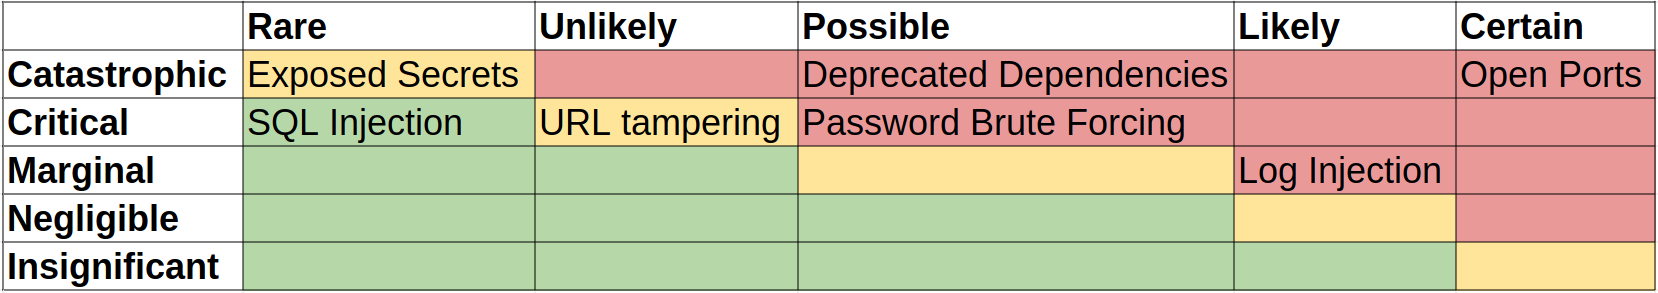
\includegraphics[width=1\textwidth]{risk-matrix.png}
    \end{center}
    \caption{https://docs.google.com/spreadsheets/d/19oRUmZ59XFHtR6ZN4iSuV3OmmRZZSoueHtJcZ4eeC3A/edit?usp=sharing}
    \label{fig:risk-matrix}
\end{figure}

\textit{\textbf{4. Action plan}}

Discuss, what we are going to do about each of the risk scenarios.
